\documentclass[fleqn]{article}
\usepackage[utf8]{inputenc}
\usepackage[margin=2.5cm]{geometry}

% bibliography
\usepackage[round, sort&compress]{natbib}
\usepackage{har2nat}
\bibliographystyle{agsm}

% custom header/footer
\usepackage{fancyhdr}
\pagestyle{fancy}
\renewcommand{\headrulewidth}{0pt}
\fancyhf{}
\rfoot{\textsf{\thepage}}
\lfoot{\textsf{Suzie Brown}}

% miscellaneous formatting
\usepackage{xcolor}
\usepackage[font=small]{caption}
\usepackage{subfig}

% tikz
\usepackage{tikz}
\usetikzlibrary{positioning}

% pseudocode
\usepackage{algorithm}
\usepackage{algorithmicx}
\usepackage{algpseudocode}

% maths
\usepackage{amsmath}
\usepackage{amssymb}
\usepackage{amsthm}
\newtheorem{corollary}{Corollary}
\theoremstyle{definition}
\newtheorem{defn}{Definition}

% useful math symbols
\newcommand{\PR}{\mathbb{P}}
\newcommand{\E}{\mathbb{E}}
\newcommand{\V}{\operatorname{Var}}
\newcommand{\eqdist}{\overset{d}{=}}
\newcommand{\I}[1]{\mathbb{I}\{#1\}}
\newcommand{\Ntoinfty}{\overset{N\to\infty}{\longrightarrow}}
\newcommand{\limNtoinfty}{\underset{N\to\infty}{\lim}}
\newcommand\indep{\protect\mathpalette{\protect\independenT}{\perp}}
\def\independenT#1#2{\mathrel{\rlap{$#1#2$}\mkern2mu{#1#2}}}

% distributions
\newcommand{\Cat}{\operatorname{Categorical}}
\newcommand{\Unif}{\operatorname{Uniform}}
\newcommand{\Mn}{\operatorname{Multinomial}}
\newcommand{\Bin}{\operatorname{Binomial}}

% project-specific commands
\newcommand{\F}{\mathcal{F}_{t-1}}
\newcommand{\vt}[2][t]{v_{#1}^{(#2)}}
\newcommand{\wt}[2][t]{w_{#1}^{(#2)}}
\newcommand{\wbar}[2][t]{\bar{w}_{#1}^{(#2)}}
\newcommand{\vttilde}[2][t]{\tilde{v}_{#1}^{(#2)}}

\title{Asymptotic analysis of genealogies induced by sequential Monte Carlo algorithms}
\author{Suzie Brown}
\date{\today}

\begin{document}
\maketitle
\thispagestyle{fancy}

\section{Introduction}
Since its introduction to the statistics literature by \citet{gordon1993}, sequential Monte Carlo (SMC) has found a huge range of applications and has become an indispensible tool to practitioners from many fields. 
It is particularly useful in applications such as target tracking, where the model has a natural sequential structure.
However, the sequential nature of SMC is helpful not only in inherently sequential settings, but in any setting where the quantity to be inferred has highly correlated components.

In these cases the more traditional Markov chain Monte Carlo methods are essentially useless because the strong dependence structure causes them to mix extremely slowly.
Conversely, SMC exploits this dependence structure to create recursive Monte Carlo algorithms that can be efficient in this difficult setting.
SMC allows a much wider class of models to be solved beyond the few cases where we can find an exact analytic solution.

The method is not without its problems, and it is one of these problems that we will examine in this work.\\

Sections \ref{sec:SMC} and \ref{sec:coalescent_theory} explain the background material on SMC and coalescent theory respectively. With these in place we are then able to explain the contribution of this work in the context of the SMC literature.
In Section \ref{sec:conditionalSMC} we present the first novel result of this work with an outline proof; the full proof is in the Appendix.
Section \ref{sec:resampling} introduces the next focus of this work, for which nothing is proved yet.
Finally we summarise future directions of the work, and its potential impact, in Section \ref{sec:discussion}.\\

%%%%
%While particle methods can be very effective for filtering, it is more difficult to apply them to smoothing because they typically suffer very badly from ancestral degeneracy in the particle genealogies.
%
%When attempting to mitigate this problem, one often encounters a trade-off between ancestral degeneracy (arising from resampling) and weight degeneracy (arising from sequential importance sampling). However, while weight degeneracy is a reasonably well-quantified problem, there exists little in the way of tools for quantifying ancestral degeneracy a priori. There have been some simulation studies attempting to cast light on the magnitude of this problem, but analytical findings remain elusive, since the complexity of the most commonly used particle methods makes it difficult to obtain any rigorous results.
%Consequently, there is a wealth of pertinent open questions in this area. This work attempts to extend a first result for a standard class of SMC algorithms to the more sophisticated algorithms which are typically used in practice.
%%%%

Throughout the document we will use the compact notation $X_{m:n}$ as shorthand for $X_m, X_{m+1}, \dots, X_n$, as well as $X_{-n} := X_0, \dots, X_{n-1}, X_{n+1}, \dots X_{N}$.
We denote falling factorial powers $(x)_a := x(x-1)\dots(x-a+1)$, with the convention $(x)_0 = 1$.

\section{Sequential Monte Carlo}\label{sec:SMC}
References for this section are \citet{doucet2001}, \citet{delmoral2006}, and \citet{doucet2009}.

\subsection{Class of models}
Although sequential Monte Carlo (SMC) methods can be applied in a much more general setting, they are particularly easy to motivate in the setting of state space models, where the ``sequential'' nature follows naturally from the discrete time steps present in the model. 
For the purposes of presenting the algorithm, let us consider a time-homogeneous state space model consisting of an unobservable discrete-time Markov process $X_{0:T}$ and observables $Y_{0:T}$, satisfying the conditional independence structure
\begin{align*}
& (X_{t+1:T} \indep X_{0:t-1}) \mid X_t \\
& (Y_t \indep Y_{-t}, X_{-t}) \mid X_t
\end{align*}
for all $t \in \{0,1,\dots, T\}$, as represented by the graphical model below.

\begin{center}
\begin{tikzpicture}
\node (yt) {$Y_t$};
\node (thet) [below=of yt] {$X_t$};
\node (yt1) [left=of yt] {$Y_{t-1}$};
\node (thet1) [below=of yt1] {$X_{t-1}$};
\node (dot1) [left=of thet1] {$\dots$};
\node (dot2) [right=of thet] {$\dots$};
\draw[->](thet.north)--(yt.south) node[midway, right] {\footnotesize{$g$}};
\draw[->](thet1.north)--(yt1.south) node[midway, right] {\footnotesize{$g$}};
\draw[->](thet1.east)--(thet.west) node[midway, above] {\footnotesize{$f$}};
\draw[->](dot1.east)--(thet1.west) node[midway, above] {\footnotesize{$f$}};
\draw[->](thet.east)--(dot2.west) node[midway, above] {\footnotesize{$f$}};
\end{tikzpicture}
\end{center}

We assume for notational convenience that $x_0,\dots,x_T$ take values in a common state space $\mathcal{X}$, and $y_0,\dots,y_T$ in a common state space $\mathcal{Y}$, but these assumptions can be dropped. 

Suppose we have the following model:
\begin{align*}
& X_0 \sim \mu(\cdot) \\
& X_{t+1} \mid (X_t = x_t) \sim f(\cdot | x_t)  \qquad t=0,\dots,T-1 \\
& Y_t \mid (X_t = x_t) \sim g(\cdot | x_t) \qquad t=0,\dots,T
\end{align*}
where $(X_t)_{t=0}^T$ is an unobservable discrete-time Markov process and the observables $(Y_t)_{t=0}^T$ satisfy $Y_t \indep \{Y_{-t}, X_{-t}\} \mid X_t$. 

We assume that the \emph{transition} and \emph{emission} kernels have densities which are denoted by $f$ and $g$ respectively, but this is not necessary in general.
We only require that we can sample from $\mu(\cdot)$ and $f(\cdot | x)$, and calculate \emph{unnormalised} potentials $g(y|x)$, for all $x,y$.

As a concrete example, let us consider the application of target tracking. Suppose we 
are using radar to track the position of an aeroplane. The true trajectory of the aeroplane is unknown and is represented by $X_{0:T}$ (perhaps a sequence of positions in $\mathbb{R}^3$), with $f$ encoding our model for how an aeroplane moves (perhaps some differential equations). What we observe is the output $Y_{0:T}$ of our radar equipment, which has some measurement uncertainty that is encoded in $g$.

\subsection{Inference in state space models}
Suppose we are in a Bayesian setting, where $\mu$ is our prior distribution at time 0, observations $y_t$ arrive sequentially, and we want to infer information about the hidden states (either on- or off-line).
The three main inference problems are:
\begin{description}
\item[Filtering] (where is it now?) $p(x_{t} | y_{0:t})$
\item[Prediction] (where will it go next?) $p(x_{t+1} | y_{0:t})$
\item[Smoothing] (where has it been?) $p(x_{0:t} | y_{0:t})$
\end{description}
In the on-line setting, we take as our prior the posterior distribution from the previous time step $t-1$, and update it using the new observation $y_t$. The inference must be fast enough to keep up with the rate of arrival of observations, so in particular the complexity of the update must not increase with $T$.
In the off-line setting, we take $\mu$ as the prior distribution, and infer the set of posteriors once all $T+1$ observations have arrived.

Prediction and filtering are essentially equivalent, because given a filtering distribution, the corresponding predictive distribution can be obtained by applying the transition kernel $f$.
Smoothing is considered a harder task because it requires us to infer many more parameters from the same amount of information; indeed the dimension of the problem increases linearly with $T$.
%In general it is not possible to infer the smoothing distributions on-line, because this would require using all of the previous observations at each time step, so the complexity would increase at each step. Algorithms that exist for on-line smoothing [REFs] are typically either approximate or computationally expensive.

In the case of linear Gaussian state space models, the posterior distributions of interest are available analytically, by way of the Kalman filter \citep{kalman1960} and Rauch-Tung-Striebel (RTS) smoother recursions \citep{rauch1965}. Recursions are also available for some other conjugate models: see for example \citet{vidoni1999}.
The other analytic case occurs if the state space of $(X_t)_{t=0}^\infty$ is finite, in which case the forward-backward algorithm \citep{baum1970} yields the exact posteriors.

\subsection{Particle approximation}
\textcolor{red}{
- Add a section including theoretical justification for SMC...?\\
- If so, rearrange to have Sec: State Space Models $\rightarrow$ Sub: Class of Models; Inference Problems; Methods (non-SMC) + Sec: SMC $\rightarrow$ Sub: SMC for SSMs; Theoretical Justification for SMC.\\
}

In more complex models such techniques are not feasible, and we are forced to resort to Monte Carlo methods.
For state space models, Markov chain Monte Carlo methods are not very effective due to the high dimension of the parameter space. But we can exploit the sequential nature of the underlying dynamics to decompose the problem into a sequence of inferences of more manageable dimension.
This is the motivation behind sequential Monte Carlo (SMC) methods.

The conditional independence structure in the model implies that the (joint) marginal distribution of the hidden states $X_{0:t}$ is given by
\begin{equation*} \label{eq:hmm_marginal}
p(x_{0:t}) = \mu(x_0) \prod_{i=1}^t f(x_i \mid x_{i-1})
\end{equation*}
and that the likelihood of the observations $y_{0:t}$ given the underlying states $x_{0:t}$ takes the form
\begin{equation*} \label{eq:hmm_likelihood}
p(y_{0:t} \mid x_{0:t}) = \prod_{i=0}^t g(y_i \mid x_i).
\end{equation*}

%The smoothing distribution $p(x_{t} | y_{0:T})$ is obtained from $p(x_{0:T} | y_{0:T})$ by marginalising. %%% what did I even mean here?
Using the conditional independence structure, we can write
\begin{align}
p(x_{0:t} | y_{0:t}) &\propto g(y_t | x_t) f(x_t | x_{t-1}) p(x_{0:t-1} | y_{0:t-1}) \label{eq:smooth_recursion}\\
&\propto \mu(x_0) g(y_0 | x_0) \prod_{i=1}^t f(x_i | x_{i-1}) g(y_i | x_i) \label{eq:smooth_recursion2}
\end{align}
for $t = 0,\dots,M$, where the one-step recursion \eqref{eq:smooth_recursion} is obtained using Bayes rule, and \eqref{eq:smooth_recursion2} is obtained by applying \eqref{eq:smooth_recursion} $t$ times. 
The filtering distribution $p(x_t | y_{0:t})$ can be obtained from \eqref{eq:smooth_recursion} by marginalising out $x_{0:t-1}$, which is straightforward if Monte Carlo samples are available.
The predictive distributions can also be derived from the smoothing distributions using
\begin{equation*}
p(x_{t+1} | y_{0:t}) \propto f(x_{t+1} | x_t) p(x_{0:t} | y_{0:t}).
\end{equation*}

SMC provides a particle method to approximate to \eqref{eq:smooth_recursion}, given a model specification and a sequence of observations. Like the underlying process, the algorithm proceeds sequentially, returning its approximation to the smoothing distribution at each time step.
This approximation is the empirical distribution of the particles:
\begin{equation}
\hat{p}(x_{0:t}|y_{0:t}) = \frac{1}{N} \sum_{i=1}^N \delta_{X_{0:t}^{(i)}}
\end{equation}
The particle approximation is justified by various convergence results - see for example \citet{delmoral2013} for details.

A generic SMC algorithm is presented in Algorithm \ref{alg:SMC}. For the state space model described above, we can take $K_{t+1}(x_t, \cdot) \equiv f(\cdot | x_t)$ and $g_{t+1}(x_t, x_{t+1}) \equiv g(y_{t+1} | x_{t+1})$.

Figure \ref{fig:SMC_vs_kalman} illustrates the particle approximation arising from such an algorithm on a linear Gaussian model, with the exact posterior for reference.

\begin{algorithm}
\caption{Standard SMC}\label{alg:SMC}
\begin{algorithmic}[1]
\Require $N, T, \mu, \{K_t\}, \{g_t\}, y_{0:T}$
\For{$i \in \{1,\dots,N\}$} 
	\State Sample $X_0^{(i)} \sim \mu(\cdot)$  \Comment initialise
	\State $w_0^{(i)} \gets \frac{g_0(X_0^{(i)})}{\sum_{j=1}^N g_0(X_0^{(j)})}$
\EndFor
\For{$t \in \{0,\dots, T-1\}$}
	\State Sample $a_t^{(1:N)} \sim $ {\footnotesize RESAMPLE}$(\{1,\dots ,N\}, \wt{1:N}$) \Comment resample particles
	\For{$i \in \{1,\dots,N\}$}
		\State Sample $X_{t+1}^{(i)} \sim K_{t+1}(X_t^{(a_t^{(i)})}, \cdot)$ \Comment propagate particles
		\State $w_{t+1}^{(i)} \gets g_{t+1}(X_t^{(a_t^{(i)})} , X_{t+1}^{(i)})$ \Comment calculate weights
	\EndFor
	\State $W \gets \sum_{j=1}^N w_{t+1}^{(j)}$
	\For{$i \in \{1,\dots, N\}$}	
		\State $w_{t+1}^{(i)} \gets \frac{1}{W}w_{t+1}^{(i)}$ \Comment normalise weights
	\EndFor
\EndFor
\end{algorithmic}
\end{algorithm}

If only the latest filtering distribution is required, we can marginalise out $\mathbf{x}_{0:t-1}$ at each step by simply throwing away the particle histories and keeping only the particle approximation $\mathbf{x}_{t}$ to the filtering distribution at the current time $t$. 
The algorithm progresses in a Markovian fashion, only ever referring to the particles at the immediately previous step, so filtering distributions can be approximated with minimal memory usage. 
If, say, the mean and variance of $X_{t} \mid y_{0:t}$ at each time $t$ are required, we can store just these summary statistics, plus the two most recent generations of particles, and throw away all other information about the particles at previous time steps. This is vital if one wishes to carry out filtering in an on-line fashion, as it prevents the memory requirements accumulating more than necessary.

The form of the {\footnotesize RESAMPLE} function in Algorithm \ref{alg:SMC} is discussed in Section \ref{sec:resampling}.

\begin{figure}
\centering
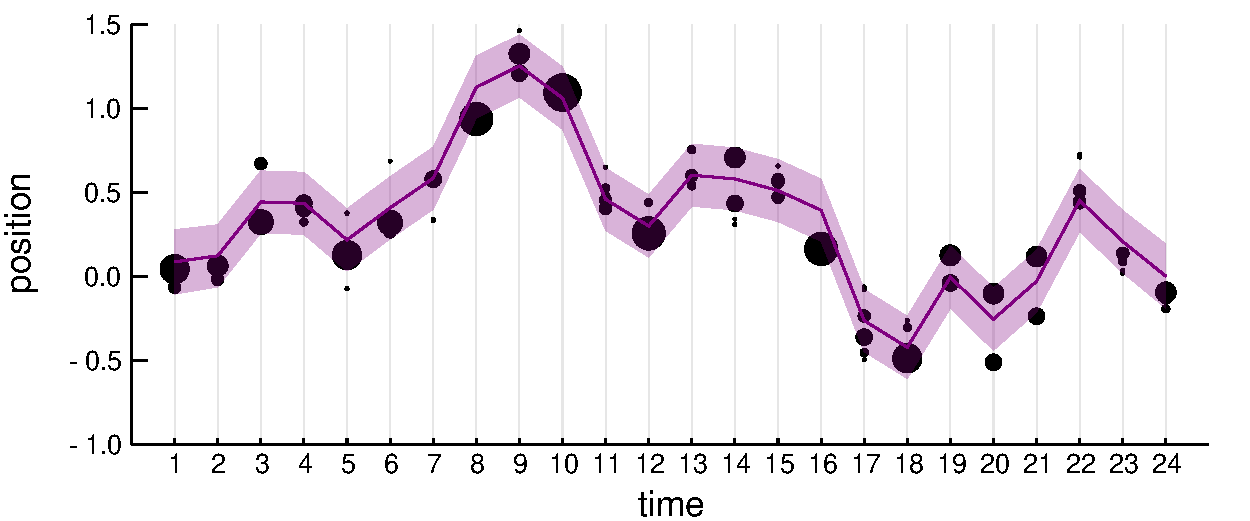
\includegraphics[width=0.9\textwidth]{smc_kalman.pdf}
\caption{SMC particles before resampling for a linear Gaussian model. The purple ribbon shows the exact posterior mode and 95\% credible interval, computed using the Kalman filter and RTS smoother. The black dots show the positions of the SMC particles, with size proportional to weight. After resampling all particles have equal weights but some are duplicated.}
\label{fig:SMC_vs_kalman}
\end{figure}


\section{Coalescent Theory}\label{sec:coalescent_theory}
\textcolor{red}{
- asymptotic coalescents for various population models\\
- time is going backwards now...\\
- Cannings model: exchangeability, also a key assumption for our SMC tings\\
- without exchangeability, can't even expect Markov process
}

\begin{defn}[\citet{mohle1998}]
Let $\mathcal{E}_n$ denote the set of equivalence relations on $\{1,\dots,n\}$.
A \emph{discrete-time coalescent} is a stochastic process $(R_t)_{t\in\mathbb{N}}$ taking values in $\mathcal{E}_n$ such that 
$R_0 = \{(1,1),(2,2),\dots,(n,n)\}$ and $\PR[R_{t+1} = \eta \mid R_{0:t-1}, R_{t} = \xi] > 0$ only if $\xi \subseteq \eta$.
\end{defn}
That is, the initial state is the trivial relation where each index is in its own equivalence class, and the only possible forward-in-time transitions are staying the same or merging some equivalence classes together.
An obvious consequence of this is that the state where all of the indices are in the same equivalence class is an absorbing state for the process.

The genealogical interpretation of the equivalence relations is that $(i,j) \in R_t$ if and only if individuals $i$ and $j$ share a common ancestor in generation $t$.

\subsection{Kingman's coalescent}
Imagine we have a population with fixed size $N$ over discrete generations, where each individual is descended from one randomly chosen individual of the previous generation. Then for each individual in the present generation, we can trace their \emph{lineage} back through the generations. 
If we trace two lineages back in time, at some generation they may descend from the same individual, at which point we say they have \emph{coalesced}. Once two lineages have coalesced they will stay together going backwards in time.
The combined lineages of $n\leq N$ of the present individuals therefore forms a tree, or several non-overlapping trees, the entirety of which we refer to as the \emph{ancestry} or \emph{genealogy} of those $n$ individuals.

Kingman's \emph{$n$-coalescent} provides a model for such genealogies. Kingman showed in \citep{kingman1982gene, kingman1982coal, kingman1982exch} that  the $n$-coalescent is the limiting process for samples from a wide class of population models as $N\to\infty$.

\begin{figure}
\centering
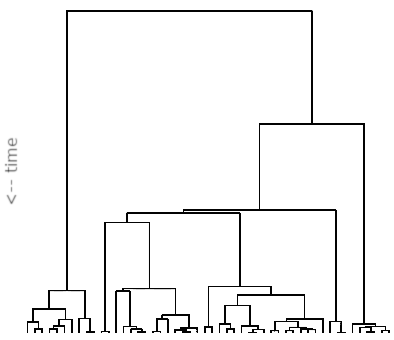
\includegraphics[width=0.6\textwidth]{kingman.png}
\caption{A realisation of Kingman's $n$-coalescent for a sample of size $n=50$. At first there are many distinct lineages, and mergers happen rapidly. Once there are fewer distinct lineages left, they take longer to merge. The process spends about half of its time with just two or three distinct lineages. \textit{(Source: Wikimedia Commons)}}
\label{fig:kingman}
\end{figure}

The defining feature of the model is that each pair of lineages merges with unit rate. This means that many coalescences occur while there are many distinct lineages present.
In particular, the $n$-coalescent can be formulated as a Poisson process where pairs of lineages coalesce independently at rate 1, with the pair to coalesce being chosen uniformly at random \citep[Section 3.2]{wakeley2009}.

In the notation of \citet{wakeley2009}, let $T_i;\, i=2,\dots,n$ be the $i^{th}$ coalescence time, that is, the length of time for which there are exactly $i$ branches in the sample genealogy. The $n$-coalescent is the process in which these times are distributed as independent Exponentials with rate $\binom{i}{2}$.

\citet{mohle1998} writes the same process in terms of the infinitesimal generator $Q$ of a Markov process on the set of equivalence relations on $n$ elements, having entries
\begin{equation*}
q_{\xi\eta} =
\begin{cases}
-\binom{b}{2} &\text{if }\xi=\eta \\
1 & \text{if }\xi \prec\eta \\
0 & \text{otherwise}
\end{cases}
\end{equation*}
where $b$ is the number of equivalence classes of $\xi$, and $\xi \prec \eta$ means that $\eta$ is a state with exactly one more pair of lineages coalesced compared to $\xi$.
 
%The \emph{Kingman coalescent} is the process on the whole population of size $N\to\infty$, such that the genealogy of any sample of size $n<N$ individuals from the present generation is an $n$-coalescent.
%%% not true - fix this!


\section{SMC genealogies as coalescents}
\textcolor{red}{
- motivate the work: see notes on back of Adam's scribbled-on copy \& commented paragraph in intro\\
- resampling viewed backwards in time: branching process $\to$ coalescent process\\
- asymptotic properties of SMC lit review: CLT, path storage, coalescence etc.\\
- the gap in knowledge that we aim to fill\\
- why the simple SSM described at start is sufficient to demonstrate coalescence\\
- how to deal with the difference between Kingman (time stops once all coalesced) and SMC genealogies (fixed time frame T)
}

\subsection{Ancestral degeneracy}
The resampling step in Algorithm \ref{alg:SMC} induces a genealogical tree.
During resampling, some particles have multiple offspring while others have none. The particles with no offspring ``die out''; they are not in the lineage of any time $T$ particle. So unless the offspring variance is low, the $N$ time $T$ particles are likely to originate from only a few distinct time $0$ ancestors.
An example of this is shown in Figure \ref{fig:WF_tree}.

\begin{figure}
\centering
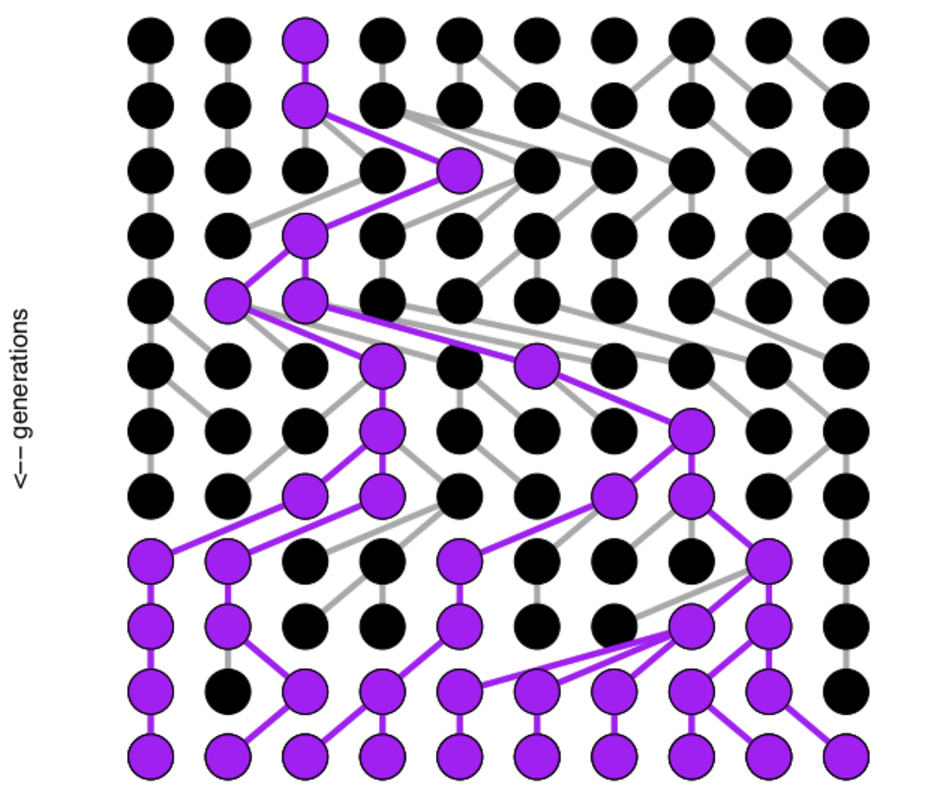
\includegraphics[width=0.8\textwidth]{eg_WF.pdf}
\caption{Genelaogical tree induced by resampling over 12 generations with $N=10$ particles. At each resampling step, any particles with no offspring ``die out''; they are not in the lineage of any time $T$ particle. In this realisation, the $N$ particles at time $T$ all originate from the same time $0$ ancestor. ``Dead'' particles/lineages are coloured black/grey, while the ``live'' tree is highlighted in purple.}
\label{fig:WF_tree}
\end{figure}

In order to estimate filtering distributions $p(x_t | y_{0:t})$, we only require a sample of particles at the current time step, so if $\mathcal{X}$ is continuous we typically have $N$ distinct positions given by the $N$ particles. Then the empirical measure has mass in $N$ locations, and the Monte Carlo error for estimating expectations under $p(x_t | y_{0:t})$ scales as $O(N^{-1/2})$ [REF].

However, we do not achieve the same performance in the case of estimating the  smoothing distributions $p(x_{0:t} | y_{0:t})$. In this case we require a sample of trajectories over times $0:t$ as opposed to a sample of particles at time $t$.
The coalescence of lineages is an unavoidable effect of resampling, and it causes more and more of these trajectories to coincide the further into the past we look.
The resulting empirical measure typically consists of $N$ distinct masses, but the marginals at early times may just consist of a single mass repeated $N$ times.
This phenomenon, known as \emph{ancestral degeneracy}, is illustrated in Figure \ref{fig:degeneracy}.

So if we are really interested in the smoothed states a long way into the past, the estimation variance will be huge. This problem was identified even in the early literature \citep{gordon1993}, where some ad hoc methods were proposed to reduce it. Since then there has been a lot of work towards mitigating ancestral degeneracy, some of which are discussed in Section \ref{sec:resampling}.\\
\textcolor{red}{
- Ancestral vs.\ weight degeneracy\\
- More discussion of general techniques to mitigate it?\\
}

\begin{figure}
\centering
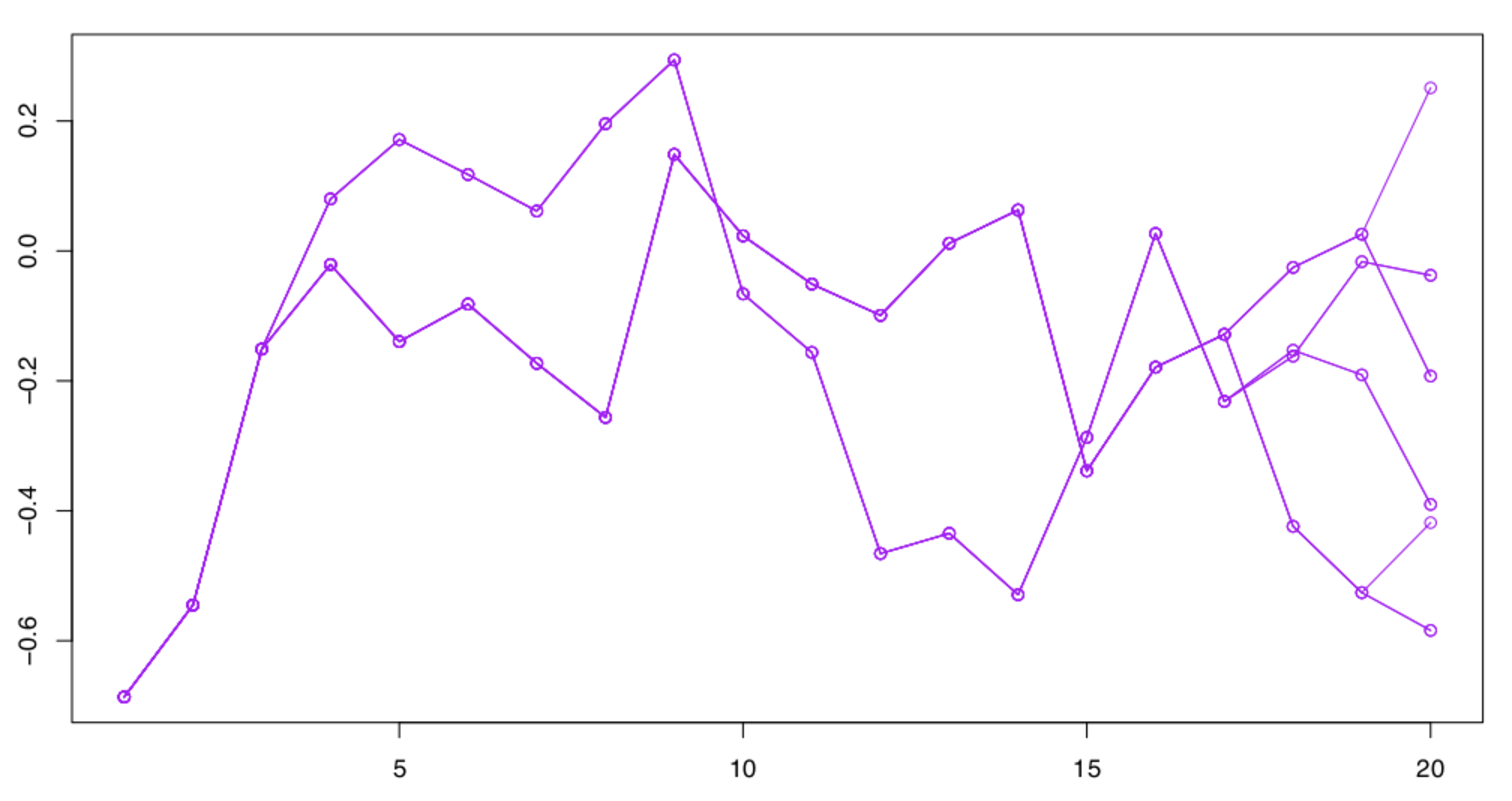
\includegraphics[width=0.8\textwidth]{degeneracy.pdf}
\caption{A sample of $N=6$ trajectories, illustrating ancestral degeneracy. At the ``present'' time there are six distinct lineages, but just three steps back they have coalesced onto only two lineages, and it takes less than 20 steps back before only one lineage remains.}
\label{fig:degeneracy}
\end{figure}

\subsection{Existing results}
\textcolor{red}{
Rewrite this section after adding details in Sec 3...
}\\
The first results showing convergence of population models to the Kingman coalescent appear in Kingman's original paper \citep{kingman1982gene} introducing the Kingman coalescent. This includes, but is not limited to, the neutral Wright-Fisher model \citep{fisher1923, fisher1930, wright1931} and the Moran model \citep{moran1958}.
It is known that a general class of exchangeable models known as neutral Cannings models converge to the Kingman coalescent \citep[Section 2.2]{etheridge2011}.
\citet{mohle1998} proved convergence for a larger class, including some non-exchangeable models.

\citet{koskela2018} presents the first application of this type of analysis to SMC genealogies. Their result relies heavily on the methods introduced by \citet{mohle1998}.
They were able to prove convergence to the Kingman coalescent for genealogies induced by standard SMC algorithms with multinomial resampling.
In the following sections we attempt to extend their result to cover some other SMC algorithms.


\section{Conditional SMC}\label{sec:conditionalSMC}
\textcolor{red}{
- Introduce particle MCMC (perhaps including basic algorithm)\\
- Then motivate conditional SMC as update in PMCMC\\
}

Conditional SMC differs from the standard algorithm in that one predetermined trajectory (that is, a sequence of particle positions and the corresponding ancestral line) is conditioned to survive all of the propagation and resampling steps. 
We will refer to this sequence as the \emph{immortal trajectory}, following the terminology used for conditioned Galton-Watson processes, and the \emph{immortal particle} will refer to the particle in a particular generation that is part of the immortal trajectory.

The conditional SMC algorithm was proposed by \citet{andrieu2010} for use in the \emph{particle Gibbs} sampler, which they introduce as part of a more general class of particle MCMC methods. 
In the particle Gibbs sampler, the standard SMC algorithm does not admit the desired target distribution, so this conditional version must be used instead.

When used as a component of the particle Gibbs algorithm, the immortal trajectory $x_{0:T}^*$ for each SMC run is sampled from the trajectories output from the previous run \citep[Section 2.4.3]{andrieu2010}. However, for our purposes we just consider a single SMC run for which the immortal trajectory is fixed.

A conditional SMC algorithm employing multinomial resampling is described in Algorithm \ref{alg:condSMC}.

\begin{algorithm}
\begin{algorithmic}[1]
\Require $N, T, \mu, \{K_t\}, \{g_t\}, y_{0:T}, x_{0:T}^*$
\For{$i \in \{1,\dots,N\}$} 
	\State Sample $X_0^{(i)} \sim \mu(\cdot)$ \Comment initialise
\EndFor
\State Sample $a_0^* \sim \Unif(\{1,\dots,N\})$
\State $X_0^{(a_0^*)} \gets x_0^*$
\For{$i \in \{1,\dots,N\}$}
	\State $w_0^{(i)} \gets \frac{g_0(X_0^{(i)})}{\sum_{j=1}^N g_0(X_0^{(j)})}$
\EndFor
\For{$t \in \{0,\dots, T-1\}$}
	\State Sample $a_t^{(1:N)} \sim \Cat(\{1,\dots,N\}, w_t^{(1:N)})$ \Comment resample particles
	\State Sample $a_{t+1}^* \sim \Unif(\{1,\dots,N\})$
	\State $a_t^{(a_{t+1}^*)} \gets a_t^*$
	\For{$i \in \{1,\dots,N\}$}
		\State Sample $X_{t+1}^{(i)} \sim K_{t+1}(X_t^{(a_t^{(i)})}, \cdot)$ \Comment propagate particles
	\EndFor
	\State $X_{t+1}^{(a_{t+1}^*)} \gets X_{t+1}^*$
	\For{$i \in \{1,\dots, N\}$}	
		\State $w_{t+1}^{(i)} \gets g_{t+1}(X_t^{(a_t^{(i)})} , X_{t+1}^{(i)})$ \Comment calculate weights
	\EndFor
	\State $W \gets \sum_{j=1}^N w_{t+1}^{(j)}$
	\For{$i \in \{1,\dots, N\}$}	
		\State $w_{t+1}^{(i)} \gets \frac{1}{W}w_{t+1}^{(i)}$ \Comment normalise weights
	\EndFor
\EndFor
\end{algorithmic}
\caption{Conditional SMC with multinomial resampling}
\label{alg:condSMC}
\end{algorithm}

In the particle Gibbs sampler, it is crucial that the conditional SMC output maintains at least two distinct trajectories. 
The immortal trajectory will of course be among the surviving trajectories, but additionally, the new immortal trajectory (for the next SMC run) is chosen from among the surviving trajectories.
Thus if all the trajectories coalesce onto the immortal trajectory, we are forced to choose the same immortal trajectory for the next run, at least for some early time steps.
One can imagine that if there was a high probability of full coalescence on each run, we could easily end up with samples from $p(x_{0:T}|y_{0:T})$ that are identical in some coordinates $0:t$, which would not lead to good results overall.

The problem can be avoided by using a sufficiently large number of particles for the fixed time window $T$ of the conditional SMC runs. This would require a priori knowledge of the coalescence mechanism, which is not available. However, Corollary \ref{thm:condSMC_kingman} could possibly provide such knowledge.
If, say, we want to ensure that the probability of all $N$ lineages coalescing is below a certain threshold, all of the relevant information is encoded in the distribution of the time to MRCA of the genealogical process. For the Kingman coalescent this distribution is known, and Corollary \ref{thm:condSMC_kingman} states that as $N\to\infty$ the genealogy is a Kingman coalescent.
The remaining question is whether the Kingman coalescent provides a reasonable approximation outside of the asymptotic regime - since in reality we simulate finitely many particles. We intend to investigate this question by way of a simulation study.

\subsection{Genealogies of conditional SMC algorithms}
In this section we calculate various quantities related to the genealogical process induced by conditional SMC with multinomial resampling. By writing these in terms of the corresponding quantities for standard SMC with multinomial resampling, we are able to apply results from \citet{koskela2018}. In this way we will show that the genealogical process converges to the Kingman coalescent, in the sense of finite-dimensional distributions, as the number of particles $N\to\infty$.

The derivations of the expressions \eqref{eq:cNtilde}, \eqref{eq:DNtilde}, \eqref{eq:cNtilde2}, along with details of the application of results from \citet{koskela2018}, are relegated to the appendix. Below is an overview of the proof.
To prove convergence to the Kingman coalescent, we must control the rates of different types of mergers. In particular, we ensure that in the large population limit (under an appropriate time-scaling), pairwise mergers happen at the correct rate, and larger mergers never occur.

Throughout the following we use tilde to indicate the conditional SMC versions of the untilded quantities relating to standard SMC, always with multinomial resampling.

Firstly, we have the expected coalescence rate:
\begin{equation}\label{eq:cNtilde}
\E[\tilde{c}_N(t) |\F] = \frac{N-2}{N} \E[c_N(t) |\F] + \frac{2}{N} \E[\wt{1} |\F]
\end{equation}
Then the expected rate of super-binary mergers (that is, more than two lineages merging simultaneously into one or more lineages) is bounded above by:
\begin{align}\label{eq:DNtilde}
\E[\tilde{D}_N(t) |\F] 
&\leq \E[D_N(t) |\F] + \frac{3}{N} \E[(\wt{1})^2 |\F] +  \frac{4}{N^2}\E[\wt{1} |\F] \notag\\
&\qquad+ \frac{4}{N}\sum_{i=2}^N \E[\wt{1}(\wt{i})^2 |\F] +\frac{2}{N^2}\sum_{i=2}^N \E[\wt{1}\wt{i} |\F] + \frac{1}{N^2} \sum_{i=2}^N \E[(\wt{i})^2 |\F] 
\end{align}
And lastly the expectation of the squared coalescence rate is bounded above by:
\begin{align}\label{eq:cNtilde2}
\E[\tilde{c}_N(t)^2 |\F] 
&\leq \E[c_N(t)^2 |\F] + \frac{4}{N}\E[(\wt{1})^3 |\F] + \frac{12}{N^2} \E[(\wt{1})^2 |\F] + \frac{4}{N(N)_2} \E[\wt{1} |\F] \notag\\
&\qquad + \frac{4}{N} \sum_{i=2}^N \E[\wt{1}(\wt{i})^2 |\F]
\end{align}
%Under conditions (18) and (19) of \citet{koskela2018},  as $N\to\infty$ the weights are $\wt{i} = O(N^{-1})$, so we have:
%\begin{align*}
%& \E[\tilde{c}_N(t) |\F] \leq \E[c_N(t) |\F] + O(N^{-2}) \\
%& \E[\tilde{D}_N(t) |\F] \leq \E[D_N(t) |\F] +O(N^{-3}) \\
%& \E[\tilde{c}_N(t)^2 |\F] \leq \E[c_N(t)^2 |\F] + O(N^{-3})
%\end{align*}
We then apply Lemma 3 of \citet{koskela2018} to obtain the more tractable expressions
\begin{align*}
& \frac{\varepsilon^4}{Na^4} + O(N^{-2}) \leq \E[\tilde{c}_N(t) |\F]  \leq \frac{a^4}{N\varepsilon^4} + O(N^{-2}) \\
& \E[\tilde{D}_N(t) |\F] \leq \frac{C}{N} \E[\tilde{c}_N(t) |\F] + O(N^{-3}) \\
& \E[\tilde{c}_N(t)^2 |\F] \leq \frac{C}{N} \E[\tilde{c}_N(t) |\F] + O(N^{-3})
\end{align*}
and define the time-scaling
\begin{equation}\label{eq:tau_tilde}
\tilde{\tau}_N(t) := \min\left\{ s\geq 1 : \sum_{r=1}^s \tilde{c}_N(r) \geq t \right\}.
\end{equation}
Then, using \citet[Lemma 2]{koskela2018}, which readily generalises to our modified quantities, we are able to verify the four conditions of \citet[Theorem 1]{koskela2018}. Finally we are able to conclude the following.

\begin{corollary}\label{thm:condSMC_kingman}
Under the conditions of \citet[Lemma 3]{koskela2018}, the genealogy of any $n$ particles from a conditional SMC algorithm with multinomial resampling converges to Kingman's $n$-coalescent in the sense of finite-dimensional distributions, under the time-scaling defined in \eqref{eq:tau_tilde}.
\end{corollary}


\section{Alternative resampling schemes}\label{sec:resampling}
\textcolor{red}{
- rewrite the intro paragraph\\
- Gerber et al's optimal scheme\\
- Del Moral's toy scheme?\\
- any other interesting properties of the various schemes\\
- properties we will require from resampling schemes, eg unbiased\\
}

There is a great deal of flexibility in the function referred to as {\footnotesize RESAMPLE} in Algorithm \ref{alg:SMC}. The most straightforward choice is multinomial resampling \citep{efron1994}, which is also the easiest to analyse. However, multinomial resampling is well known to be sub-optimal in terms of the resulting Monte Carlo variance, and is rarely used in practice. For instance, \citet{douc2005} proves that both residual resampling and stratified resampling yield lower variance. 
In this section we will present some resampling schemes that claim to perform better than multinomial resampling.

\subsection{Multinomial resampling}
Multinomial resampling \citep{efron1994} is one of the simplest resampling schemes, and the one first appearing in the literature.
 
The parental indices are chosen independently from $\{1, \dots, N\}$, each with probability given by the weight of the corresponding particle $\wt{i}$. 
That is, 
\begin{equation*}
a_t^{(1:N)} \sim \Cat(\{1,\dots, N\}, \wt{1:N}) .
\end{equation*}
This implies the joint distribution of the offspring counts is 
\begin{equation*}
\vt{1:N} \eqdist \operatorname{Multinomial}(N, \wt{1:N}) .
\end{equation*}
Note that in this case the parental indices are chosen independently, but the resulting offspring counts are negatively correlated.

In practice, a common way to sample the parental indices is the following: divide the unit interval into $N$ subintervals each of which will correspond to a certain index $i$ and has length equal to the weight $\wt{i}$; then draw $N$ samples from $\Unif(0,1)$ and classify them according to which of these subintervals they fall in. This is illustrated in Figure \ref{fig:resampling_mn}.

\subsection{Residual resampling}
Residual resampling is described in \citet{liu1998} and also in \citet{whitley1994} where it is called ``remainder stochastic sampling''.

Each particle $x_{t}^{(i)}$ is deterministically assigned $\lfloor N \wt{i} \rfloor$ offspring, and the remaining $R := N- \sum \lfloor N w_{t}^{(i)} \rfloor$ offspring are assigned multinomially in proportion to the unaccounted-for weight. 
This yields offspring counts
\begin{equation*}
\vt{1:N} \eqdist \lfloor N \wt{1:N} \rfloor +  \operatorname{Multinomial}(R, (N \wt{1:N} - \lfloor N \wt{1:N}\rfloor)/R) .
\end{equation*}
The deterministic part ensures that every particle with weight $>1/N$ is guaranteed to survive. This is a desirable property as it prevents the random loss of high-weighted particles.

\subsection{Stratified resampling}
Stratified resampling is introduced in \cite{kitagawa1996}.

The scheme proceeds like Multinomial resampling, except that the Uniform samples that are fed in to do the Categorical sampling are produced in a different way.
Instead of sampling $N$ independent numbers from $\operatorname{U}(0,1)$, one number is sampled uniformly from each subinterval of length $1/N$. 
That is, 
\begin{equation*}
U_i \sim \Unif \left(\frac{i-1}{N}, \frac{i}{N} \right) .
\end{equation*}
(Of course this means that the offspring distribution is no longer Multinomial, since parental indices are not chosen independently.)
This scheme ensures that the samples are ``well spread out'', again reducing the probability of randomly losing high-weighted particles.
The method is illustrated in Figure \ref{fig:resampling_stratified}.

\subsection{Systematic resampling}
Systematic resampling is described in \citet{carpenter1999} and also in \citet{whitley1994} where it is called ``stochastic universal sampling''.

Like stratified resampling, it constitutes a change to the random number generator for sampling from the Categorical distriubtion. 
In this scheme, only one Uniform sample is drawn, $U \sim \operatorname{U}(0,1/N)$, and the other $N-1$ samples are generated deterministically by setting
\begin{equation*}
U_i = U + \frac{i-1}{N}
\end{equation*}
for each $i \in \{1, \dots, N\}$.
This scheme again ensures the random numbers are ``well spread out'', even more so than with stratified resampling.
The method is illustrated in Figure \ref{fig:resampling_systematic}.

Systematic resampling is often preferred among practitioners because it is extremely easy to implement and also computationally efficient, requiring only one random number to be generated.

\begin{figure}
\centering
\subfloat[Multinomial resampling]{
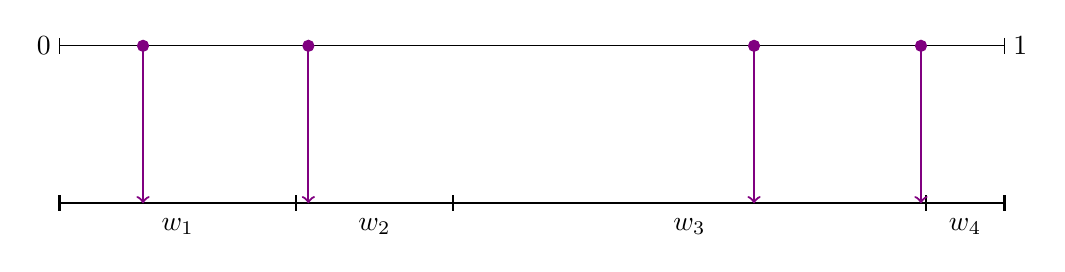
\begin{tikzpicture}
%parallel lines
\draw[thick] (0,0) -- (12,0);
\draw (0,2) -- (12,2);
% tick marks at ends
\draw[thick] (0,0.1) --(0,-0.1);
\draw[thick] (12,0.1) --(12,-0.1);
\draw (0,2.1) --(0,1.9);
\draw (12,2.1) --(12,1.9);
% tick marks indicating weights
\draw[thick] (3,0.1) --(3,-0.1);
\draw[thick] (5,0.1) --(5,-0.1);
\draw[thick] (11,0.1) --(11,-0.1);
% weight labels
\node at (1.5,-0.3) {$w_1$};
\node at (4,-0.3) {$w_2$};
\node at (8,-0.3) {$w_3$};
\node at (11.5,-0.3) {$w_4$};
% endpoint labels
\node at (-0.2,2) {$0$};
\node at (12.2,2) {$1$};
% uniform points
\filldraw[violet] (10.94,2) circle (2pt);
\filldraw[violet] (1.06,2) circle (2pt);
\filldraw[violet] (8.82,2) circle (2pt);
\filldraw[violet] (3.16,2) circle (2pt);
% arrows from random points
\draw[thick, violet, ->] (10.94,2) -- (10.94,0);
\draw[thick, violet, ->] (1.06,2) -- (1.06,0);
\draw[thick, violet, ->] (8.82,2) -- (8.82,0);
\draw[thick, violet, ->] (3.16,2) -- (3.16,0);
\end{tikzpicture}
\label{fig:resampling_mn}
}\\
\subfloat[Stratified resampling]{
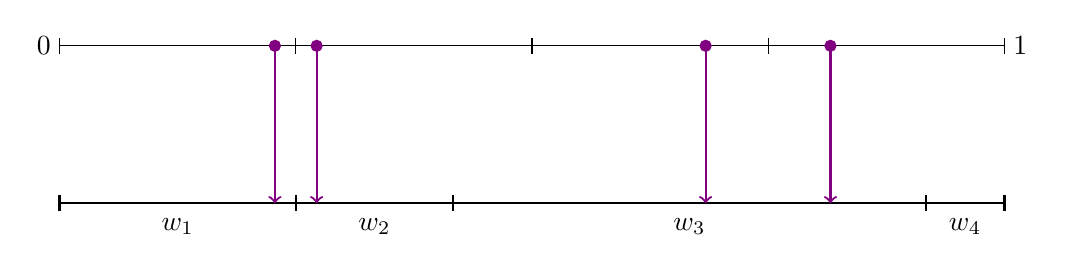
\begin{tikzpicture}
%parallel lines
\draw[thick] (0,0) -- (12,0);
\draw (0,2) -- (12,2);
% tick marks at ends
\draw[thick] (0,0.1) --(0,-0.1);
\draw[thick] (12,0.1) --(12,-0.1);
\draw (0,2.1) --(0,1.9);
\draw (12,2.1) --(12,1.9);
% tick marks indicating weights
\draw[thick] (3,0.1) --(3,-0.1);
\draw[thick] (5,0.1) --(5,-0.1);
\draw[thick] (11,0.1) --(11,-0.1);
% tick marks indicating sampling intervals:
\draw (3,2.1) --(3,1.9);
\draw (6,2.1) --(6,1.9);
\draw (9,2.1) --(9,1.9);
% weight labels
\node at (1.5,-0.3) {$w_1$};
\node at (4,-0.3) {$w_2$};
\node at (8,-0.3) {$w_3$};
\node at (11.5,-0.3) {$w_4$};
% endpoint labels
\node at (-0.2,2) {$0$};
\node at (12.2,2) {$1$};
% stratified points
\filldraw[violet] (2.735,2) circle (2pt);
\filldraw[violet] (3.265,2) circle (2pt);
\filldraw[violet] (8.205,2) circle (2pt);
\filldraw[violet] (9.79,2) circle (2pt);
% arrows from random points
\draw[thick, violet, ->] (2.735,2) -- (2.735,0);
\draw[thick, violet, ->] (3.265,2) -- (3.265,0);
\draw[thick, violet, ->] (8.205,2) -- (8.205,0);
\draw[thick, violet, ->] (9.79,2) -- (9.79,0);
\end{tikzpicture}
\label{fig:resampling_stratified}
}\\
\subfloat[Systematic resampling]{
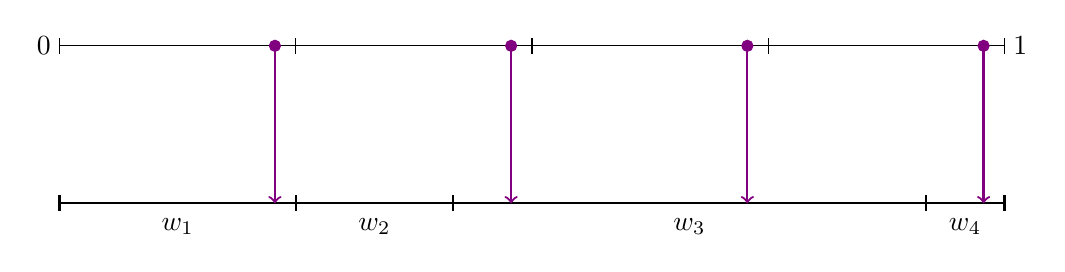
\begin{tikzpicture}
%parallel lines
\draw[thick] (0,0) -- (12,0);
\draw (0,2) -- (12,2);
% tick marks at ends
\draw[thick] (0,0.1) --(0,-0.1);
\draw[thick] (12,0.1) --(12,-0.1);
\draw (0,2.1) --(0,1.9);
\draw (12,2.1) --(12,1.9);
% tick marks indicating weights
\draw[thick] (3,0.1) --(3,-0.1);
\draw[thick] (5,0.1) --(5,-0.1);
\draw[thick] (11,0.1) --(11,-0.1);
% tick marks indicating sampling intervals:
\draw (3,2.1) --(3,1.9);
\draw (6,2.1) --(6,1.9);
\draw (9,2.1) --(9,1.9);
% weight labels
\node at (1.5,-0.3) {$w_1$};
\node at (4,-0.3) {$w_2$};
\node at (8,-0.3) {$w_3$};
\node at (11.5,-0.3) {$w_4$};
% endpoint labels
\node at (-0.2,2) {$0$};
\node at (12.2,2) {$1$};
% stratified points
\filldraw[violet] (2.735,2) circle (2pt);
\filldraw[violet] (5.735,2) circle (2pt);
\filldraw[violet] (8.735,2) circle (2pt);
\filldraw[violet] (11.735,2) circle (2pt);
% arrows from random points
\draw[thick, violet, ->] (2.735,2) -- (2.735,0);
\draw[thick, violet, ->] (5.735,2) -- (5.735,0);
\draw[thick, violet, ->] (8.735,2) -- (8.735,0);
\draw[thick, violet, ->] (11.735,2) -- (11.735,0);
\end{tikzpicture}
\label{fig:resampling_systematic}
}\\
\caption{Illustration of the way parental indices are sampled in three different resampling schemes. For this example $N=4$ and the weights are $\wt{1:4} = \frac{1}{N}(1,\frac{2}{3},2,\frac{1}{3})$. In each case the indices are assigned by sampling from $\Unif(0,1)$ and seeing which subinterval the samples land in, where the length of the subinterval corresponding to each index is given by its weight. The same $\Unif(0,1)$ samples are used in each case.\\
\textbf{(a)} For Multinomial resampling, we just sample $N$  independent $\Unif(0,1)$ random variables. In this example the sampled offspring counts are $(1,1,2,0)$.\\
\textbf{(b)} For stratified resampling, the $\Unif(0,1)$ samples are transformed to Uniform draws from the intervals (0,0.25), (0.25,0.5), (0.5, 0.75), (0.75,1). In this example the sampled offspring counts are $(1,1,2,0)$.\\
\textbf{(c)} For systematic resampling, we use only the first draw and transform as in (b) to get a sample from $\Unif(0,0.25)$. For the subsequent draws, we just add 0.25 each time to obtain a sample in each interval. In this example the sampled offspring counts are $(1,0,2,1)$.}
\end{figure}

\subsection{Remarks on performance}
\subsubsection{Support of offspring numbers}
First consider the support of the marginal offspring distributions in each scheme, given the corresponding weight. Condition on the $i^{th}$ weight lying in the interval $\wt{i} \in [k/N, (k+1)/N]$, but leave the other weights unknown. By considering the best and worst cases for each scheme, we have: 
\begin{description}
\item[Multinomial:] $\vt{i} \in \{0,\dots, N\}$
\item[Residual:] $\vt{i} \in \{k,\dots, N\}$
\item[Stratified:] $\vt{i} \in \{k-1, k+2\}$
\item[Systematic:] $\vt{i} \in \{k, k+1\}$
\end{description}
We see that multinomial resampling allows the possibility of very good particles having $0$ offspring, and of very bad particles having $N$ offspring (although the probabilities associated to these events are low).
Residual resampling ensures that good particles do not die out, but still allows bad particles to possibly have many offspring.
Stratified resampling is more restrictive, although it allows the possibility of a particle with weight $>1/N$ leaving no offspring.
Systematic resampling is more restrictive still, allowing the number of offspring of each particle to vary only by one.

\subsubsection{Permutation invariance}
A strange property of stratified and systematic resampling is that they are sensitive to the order in which the subintervals are placed. For example, in Figures \ref{fig:resampling_stratified} and \ref{fig:resampling_systematic} if the intervals $w_2$ and $w_4$ were swapped, the number of offspring assigned to particles 2 and 4 would be swapped in each case. 
We can also see that because $w_1$ has weight $\geq 1/N$ and is placed first, it is guaranteed at least one offspring.

This property can lead to pathological behaviour, but is easily avoided by applying a random permutation to the order of the subintervals.

\subsubsection{Equal weights}
Suppose we somehow end up in the situation where all the weights are equal (i.e.\ $\wt{i} = 1/N$ for all $i$).
In this case, residual resampling will result in a deterministic assignment only: each particle will be assigned one offspring, and there will be no remainder left to assign randomly. This behaviour cannot be avoided, however the event that all weights are equal typically has zero measure.

In fact, stratified and systematic resampling will have the same result: the intervals for sampling will correspond exactly to the weighted subintervals, so no matter which random numbers are sampled, exactly one will fall in each subinterval.

In the case of stratified resampling this behaviour can be avoided by shifting the sampling intervals by a random amount. In fact this random shift is inherent in all of the resampling schemes as described by \citet{whitley1994}; he imagines subdivisions of a circle rather than an interval, and then ``spins the roulette wheel'' around it.

\section{Discussion}\label{sec:discussion}
\textcolor{red}{
- results so far\\
- impact of this work: to practitioners, to enriching the SMC literature, interpretation within pop gen.\\
- future directions
}

\appendix
\section{Proof of Corollary \ref{thm:condSMC_kingman}}
In the derivation of \eqref{eq:cNtilde} -- \eqref{eq:cNtilde2} we will make extensive use of the formula for factorial moments of the multinomial distribution given in \citet[p.67]{mosimann1962}:
\begin{equation} \label{eq:mn_moments}
\E[(X_i)_a(X_j)_b] = (n)_{a+b}\, p_i^a p_j^b
\end{equation}
where $(X_1,\dots X_k) \sim \Mn(n, \mathbf{p})$.
To apply this formula we need to write everything in terms of falling factorial powers. The required conversions are summarised in Table \ref{tab:fact_powers}.

In standard SMC with multinomial resampling, the marginal offspring distributions, conditioned on the filtration $\F$ generated by the previous offspring counts, are
\begin{equation*}
\vt{i} \eqdist \Bin (N, \wt{i}), \qquad i=1,\dots,N
\end{equation*}
where $\vt{i}$ is the number of offspring in generation $t+1$ of the $i$th particle in generation $t$, $N$ is the number of particles and $\wt{i}$ is the weight associated with the $i$th particle in generation $t$.

In conditional SMC we condition on the immortal trajectory surviving each resampling step. By exchangeability we can set without loss of generality that the immortal trajectory consists of particle 1 in each generation. At each resampling step, particle 1 must therefore choose particle 1 as its parent, while the remaining $N-1$ offspring are assigned multinomially to the $N$ possible parents. The marginal offspring distributions are then
\begin{align*}
& \vttilde{1} \eqdist 1 + \Bin(N-1, \wt{1}) \\
& \vttilde{i} \eqdist \Bin(N-1, \wt{i}), \qquad i=2,\dots,N.
\end{align*}
First let us consider the pair-merger rate
\begin{equation*}
c_N(t) := \frac{1}{(N)_2} \sum_{i=1}^{N} (\vt{i})_2.
\end{equation*}
For standard SMC the expected value is, using the tower rule,
\begin{equation*}
\E[c_N(t) |\F] 
= \frac{1}{(N)_2} \sum_{i=1}^{N} \E\left[ \E[ (\vt{i})_2 ] |\F \right]
=\frac{1}{(N)_2} \sum_{i=1}^{N} \E\left[(N)_2 (\wt{i})^2 |\F \right] 
= \sum_{i=1}^{N} \E\left[(\wt{i})^2 |\F \right]
\end{equation*}
as stated in \citet[Remark 3]{koskela2018}.
In the case of conditional SMC we separate the first term (corresponding to the immortal particle) from the sum to get
\begin{align*}
\E[\tilde{c}_N(t) |\F] &= \frac{1}{(N)_2} \sum_{i=1}^{N} \E\left[ (\vttilde{i})_2 |\F \right] 
= \frac{1}{(N)_2} \E\left[ (\vttilde{1})_2 |\F \right] + \frac{1}{(N)_2}\sum_{i=2}^{N} \E\left[ (\vttilde{i})_2 |\F \right] \\
&= \frac{1}{(N)_2} \left\{ (N-1)_2\E[(\wt{1})^2 |\F] + 2(N-1)\E[\wt{1} |\F] + \sum_{i=2}^{N} (N-1)_2\E[(\wt{i})^2 |\F] \right\}\\
&= \frac{(N-1)_2}{(N)_2} \sum_{i=1}^{N} \E[(\wt{i})^2 |\F] + \frac{2(N-1)}{(N)_2} \E[\wt{1} |\F] \\
&= \frac{N-2}{N} \E[c_N(t) |\F] + \frac{2}{N} \E[\wt{1} |\F]
\end{align*}
which gives us \eqref{eq:cNtilde}.

\begin{table}
\centering
\begin{tabular}{r c l}
\hline
$x$ & $=$ & $(x)_1$ \\
$x^2$ & $=$ & $(x)_2 + (x)_1$ \\
$x^3$ & $=$ & $(x)_3 + 3(x)_2 + (x)_1$ \\
$x^4$ & $=$ & $(x)_4 + 6(x)_3 + 7(x)_2 + (x)_1$ \\
\hline
$xy$ & $=$ & $(x)_1(y)_1$ \\
$x^2y$ & $=$ & $(x)_2(y)_1 + (x)_1(y)_1$ \\
$xy^2$ & $=$ & $(x)_1(y)_2 + (x)_1(y)_1$ \\
$x^2y^2$ & $=$ & $(x)_2(y)_2 + (x)_2(y)_1 + (x)_1(y)_2 +  (x)_1(y)_1$ \\
\hline
$(x+1)_2$ & $=$ & $(x)_2 + 2(x)_1$ \\
$(x+1)^2$ & $=$ & $(x)_2 + 3(x)_1 + 1$ \\
$(x+1)_2(x+1)$ & $=$ & $(x)_3 + 5(x)_2 + 4(x)_1$ \\
$(x+1)_2^2$ & $=$ & $(x)_4 + 8(x)_3 + 14(x)_2 + 4(x)_1$ \\
\hline
\end{tabular}
\caption{Conversion of ordinary powers into falling factorial powers}
\label{tab:fact_powers}
\end{table}

An upper bound on the rate of super-binary mergers is given by
\begin{equation*}
D_N(t) := \frac{1}{N(N)_2} \sum_{i=1}^N (\vt{i})_2 \left( \vt{i} + \frac{1}{N} \sum_{j\neq i} (\vt{j})^2 \right).
\end{equation*}
In the standard case this quantity has expectation
\begin{align*}
\E[D_N(t) |\F] &= \frac{1}{N(N)_2} \sum_{i=1}^N \left\{ (N)_3\E[(\wt{i})^3 |\F] + 2(N)_2\E[(\wt{i})^2 |\F] \right\} \\
&\qquad + \frac{1}{N^2(N)_2} \sum_{i=1}^N \sum_{j\neq i} \left\{ (N)_4\E[(\wt{i})^2(\wt{j})^2 |\F] + (N)_3\E[(\wt{i})^2\wt{j} |\F] \right\}
\end{align*}
while in the conditional case, again separating the terms involving particle 1,
\begin{align*}
\tilde{D}_N(t) &= \frac{1}{N(N)_2} (\vttilde{1})_2 \left(\vttilde{1} + \frac{1}{N} \sum_{j\neq 1} (\vttilde{j})^2 \right)
+ \frac{1}{N(N)_2} \sum_{i\neq 1} (\vttilde{i})_2 \left( \vttilde{i} + \frac{1}{N}(\vttilde{1})^2 + \frac{1}{N} \sum_{1\neq j\neq i} (\vttilde{j})^2 \right)\\
&= \frac{1}{N(N)_2} \left\{ (\vttilde{1})_2\vt{1} + \frac{1}{N}\sum_{j\neq 1} (\vttilde{1})_2(\vttilde{j})^2 + \frac{1}{N}\sum_{i\neq 1} (\vttilde{i})_2(\vttilde{1})^2 \right\} \\
&\qquad + \frac{1}{N(N)_2} \sum_{i\neq 1} \left\{ (\vttilde{i})_2\vttilde{i} + \frac{1}{N}\sum_{1\neq j\neq i} (\vttilde{i})_2(\vttilde{j})^2 \right\} \\
&= \frac{1}{N(N)_2} \left\{ (\vttilde{1})_2\vttilde{1} + \frac{1}{N}\sum_{i\neq 1} \left( (\vttilde{1})_2(\vttilde{i})^2 + (\vttilde{i})_2(\vttilde{1})^2 \right) \right\} \\
&\qquad + \frac{1}{N(N)_2} \sum_{i\neq 1} \left\{ (\vttilde{i})_3 + 2(\vttilde{i})_2 + \frac{1}{N}\sum_{1\neq j\neq i} \left( (\vttilde{i})_2(\vttilde{j})_2 + (\vttilde{i})_2\vttilde{j} \right) \right\}
\end{align*}
and so by applying the moments from \eqref{eq:mn_moments} and Table \ref{tab:fact_powers} we find the expectation
\begin{align*}
&\E[\tilde{D}_N(t) |\F]= \\ 
&= \frac{1}{N(N)_2} \left\{ (N-1)_3\E[(\wt{1})^3 |\F] + 5(N-1)_2\E[(\wt{1})^2 |\F] +  4(N-1)\E[\wt{1} |\F] \right\} \\
&\qquad + \frac{1}{N^2(N)_2} \sum_{i=2}^N \left\{ 2(N-1)_4\E[(\wt{1})^2(\wt{i})^2 |\F] + (N-1)_3 \E[(\wt{1})^2\wt{i} |\F] \right.\\
&\qquad\qquad + 5(N-1)_3\E[\wt{1}(\wt{i})^2 |\F] 
 \left. +2(N-1)_2\E[\wt{1}\wt{i} |\F] + (N-1)_2\E[(\wt{i})^2 |\F] \right\} \\
&\qquad + \frac{1}{N(N)_2} \sum_{i=2}^N \left\{ 
(N-1)_3\E[(\wt{i})^3 |\F] + 2(N-1)_2\E[(\wt{i})^2 |\F] \right\} \\
&\qquad + \frac{1}{N^2(N)_2} \sum_{i=2}^N \sum_{1\neq j\neq i} \left\{ (N-1)_4\E[(\wt{i})^2(\wt{j})^2 |\F] + (N-1)_3\E[(\wt{i})^2\wt{j} |\F] \right\} \\
&= \frac{1}{N(N)_2} \sum_{i=1}^N \left\{ 
(N-1)_3\E[(\wt{i})^3 |\F] + 2(N-1)_2\E[(\wt{i})^2 |\F] \right\} \\
&\qquad + \frac{1}{N^2(N)_2} \sum_{i=1}^N \sum_{j\neq i} \left\{ (N-1)_4\E[(\wt{i})^2(\wt{j})^2 |\F] + (N-1)_3\E[(\wt{i})^2\wt{j} |\F] \right\} \\
&\qquad + \frac{1}{N(N)_2}\left\{ 3(N-1)_2\E[(\wt{1})^2 |\F] +  4(N-1)\E[\wt{1} |\F] \right\} \\
&\qquad+ \frac{1}{N^2(N)_2}\sum_{i=2}^N \left\{ 4(N-1)_3\E[\wt{1}(\wt{i})^2 |\F]
+2(N-1)_2\E[\wt{1}\wt{i} |\F] + (N-1)_2\E[(\wt{i})^2 |\F] \right\} \\
&\leq \E[D_N(t) |\F] + \frac{1}{N(N)_2} \left\{3(N-1)_2\E[(\wt{1})^2 |\F] +  4(N-1)\E[\wt{1} |\F] \right\} \\
&\qquad+ \frac{1}{N^2(N)_2}\sum_{i=2}^N \left\{ 4(N-1)_3\E[\wt{1}(\wt{i})^2 |\F] +2(N-1)_2\E[\wt{1}\wt{i} |\F] + (N-1)_2\E[(\wt{i})^2 |\F] \right\} \\
&\leq \E[D_N(t) |\F] + \frac{3}{N} \E[(\wt{1})^2 |\F] +  \frac{4}{N^2}\E[\wt{1} |\F] \\
&\qquad+ \frac{4}{N}\sum_{i=2}^N \E[\wt{1}(\wt{i})^2 |\F] +\frac{2}{N^2}\sum_{i=2}^N \E[\wt{1}\wt{i} |\F] + \frac{1}{N^2} \sum_{i=2}^N \E[(\wt{i})^2 |\F] 
\end{align*}
The second line of the first equality relies on multiplying the relevant terms in Table \ref{tab:fact_powers}. For the second equality we recombine the terms in particle 1 into the sum. The inequalities follow by bounding e.g.\ $N-1$ by $N$, and identifying the first two lines with $\E[D_N(t) |\F]$. This gives us the inequality \eqref{eq:DNtilde}.

We also need control of the squared coalescence rate:
\begin{align*}
c_N(t)^2 &= \frac{1}{(N)_2^2} \left( \sum_{i=1}^N (\vt{i})_2\right)^2 = \frac{1}{(N)_2^2} \left\{ \sum_{i=1}^N \E[(\vt{i})_2^2] + \sum_{i=1}^N\sum_{j\neq i} \E[(\vt{i})_2(\vt{j})_2] \right\}
\end{align*}
A bound on its expected value is proved in \citet{koskela2018}, but here we will use a different, more explicit bound to allow direct comparison between the standard and conditional cases.
For standard SMC we have:
\begin{align*}
\E[c_N(t)^2 |\F] &= \frac{1}{(N)_2^2} \left\{ (N)_4 \sum_{i=1}^N \E[(\wt{i})^4 |\F] + 4(N)_3 \sum_{i=1}^N \E[(\wt{i})^3 |\F] + 2(N)_2 \sum_{i=1}^N \E[(\wt{i})^2 |\F] \right\} \\
&\qquad + \frac{1}{(N)_2^2}(N)_4 \sum_{i=1}^N\sum_{j\neq i} \E[(\wt{i})^2(\wt{j})^2 |\F] \\
&= \frac{1}{(N)_2} \left\{ (N-2)_2 \sum_{i=1}^N \E[(\wt{i})^4 |\F] + 4(N-2) \sum_{i=1}^N \E[(\wt{i})^3 |\F] + 2 \sum_{i=1}^N \E[(\wt{i})^2 |\F] \right. \\
&\hspace{230pt}+ \left. (N-2)_2 \sum_{i=1}^N\sum_{j\neq i} \E[(\wt{i})^2(\wt{j})^2 |\F] \right\}
\end{align*}
For conditional SMC, we again separate the terms involving particle 1:
\begin{align*}
\tilde{c}_N(t)^2 &= \frac{1}{(N)_2^2} \left\{ \sum_{i=1}^N \E[(\vttilde{i})_2^2] 
+ \sum_{i=1}^N\sum_{j\neq i} \E[(\vttilde{i})_2(\vttilde{j})_2] \right\} \\
&= \frac{1}{(N)_2^2} \left\{ \sum_{i=2}^N \E[(\vttilde{i})_2^2] +\E[(\vttilde{1})_2^2] 
+ \sum_{i=2}^N\sum_{1\neq j\neq i} \E[(\vttilde{i})_2(\vttilde{j})_2] + 2\sum_{i=2}^N \E[(\vttilde{1})_2(\vttilde{i})_2] \right\} \\
\end{align*}
and then use the same techniques as for $\tilde{D}_N(t)$ to calculate the expectation:
\begin{align*}
&\E[\tilde{c}_N(t)^2 |\F]= \\ 
&= \frac{1}{(N)_2^2} \left\{ (N-1)_4 \sum_{i=2}^N \E[(\wt{i})^4 |\F] + 4(N-1)_3 \sum_{i=2}^N \E[(\wt{i})^3 |\F] + 2(N-1)_2 \sum_{i=2}^N \E[(\wt{i})^2 |\F] \right\}  \\
&\qquad + \frac{1}{(N)_2^2} \left\{ (N-1)_4\E[(\wt{1})^4 |\F] + 8(N-1)_3\E[(\wt{1})^3 |\F] + 14(N-1)_2\E[(\wt{1})^2 |\F] \right\} \\
&\qquad +  \frac{1}{(N)_2^2}4(N-1)\E[\wt{1} |\F]
+ \frac{1}{(N)_2^2}  (N-1)_4 \sum_{i=2}^N \sum_{1\neq j \neq i} \E[(\wt{i})^2(\wt{j})^2 |\F] \\
&\qquad +\frac{2}{(N)_2^2} \sum_{i=2}^N \left( (N-1)_4 \E[(\wt{1})^2(\wt{i})^2 |\F] + 2(N-1)_3 \E[\wt{1}(\wt{i})^2 |\F] \right) \\
&= \frac{1}{(N)_2^2} \left\{ (N-1)_4 \sum_{i=1}^N \E[(\wt{i})^4 |\F] + 4(N-1)_3 \sum_{i=1}^N \E[(\wt{i})^3 |\F] + 2(N-1)_2 \sum_{i=1}^N \E[(\wt{i})^2 |\F] \right\} \\
&\qquad + \frac{(N-1)_4}{(N)_2^2} \sum_{i=1}^N\sum_{j\neq i} \E[(\wt{i})^2(\wt{j})^2 |\F] \\
&\qquad +\frac{1}{(N)_2^2} \left\{ 4(N-1)_3 \E[(\wt{1})^3 |\F] + 12(N-1)_2\E[(\wt{1})^2 |\F] + 4(N-1)\E[\wt{1} |\F] \right\} \\
&\qquad +\frac{1}{(N)_2^2} \left\{ 4(N-1)_3 \sum_{i=2}^N \E[\wt{1}(\wt{i})^2 |\F] \right\} \\
&\leq  \E[c_N(t)^2 |\F] + \frac{1}{(N)_2^2} \left\{4(N-1)_3 \E[(\wt{1})^3 |\F] + 12(N-1)_2 \E[(\wt{1})^2 |\F] \right\}\\
&\qquad +\frac{1}{(N)_2^2} \left\{ 4(N-1)\E[\wt{1} |\F]
+ 4(N-1)_3 \sum_{i=2}^N \E[\wt{1}(\wt{i})^2 |\F] \right\} \\
&\leq \E[c_N(t)^2 |\F] + \frac{4}{N}\E[(\wt{1})^3 |\F] + \frac{12}{N^2} \E[(\wt{1})^2 |\F] + \frac{4}{N(N)_2} \E[\wt{1} |\F]\\
&\qquad + \frac{4}{N} \sum_{i=2}^N \E[\wt{1}(\wt{i})^2 |\F]
\end{align*}
The conditions (18) and (19) of \citet[Lemma 3]{koskela2018} give us control over the weights so that we have $\wt{i} = O(1)$ for all $i$. Under these conditions, in the limit as $N\to\infty$, the three modified expectations derived above simplify to:
\begin{align*}
& \E[\tilde{c}_N(t) |\F] \leq \E[c_N(t) |\F] + O(N^{-2}) \\
& \E[\tilde{D}_N(t) |\F] \leq \E[D_N(t) |\F] +O(N^{-3}) \\
& \E[\tilde{c}_N(t)^2 |\F] \leq \E[c_N(t)^2 |\F] + O(N^{-3})
\end{align*}
This shows that each of these quantities for conditional SMC is bounded above by the corresponding standard SMC quantity, plus some vanishing error term. This will allow us to apply \citet[Theorem 1]{koskela2018}, as we will show in the following.

Next we apply the result of \citet[Lemma 3]{koskela2018}, so that for our modified quantity $\tilde{c}_N(t)$ we have the upper bound:
\begin{align}\label{eq:cN_upper}
\E[\tilde{c}_N(t) |\F] &= \frac{N-2}{N} \E[c_N(t) |\F] + \frac{2}{N} \E[\wt{1} |\F] \notag\\
& \leq \E[c_N(t) |\F] + \frac{2}{N} \E[\wt{1} |\F] \notag\\
&\leq \frac{a^4}{N\varepsilon^4} +  \frac{2}{N} \E[\wt{1} |\F] \notag\\
&= \frac{a^4}{N\varepsilon^4} + O(N^{-2})
\end{align}
and lower bound:
\begin{align}\label{eq:cN_lower}
\E[\tilde{c}_N(t) |\F] &= \frac{N-2}{N} \E[c_N(t) |\F] + \frac{2}{N} \E[\wt{1} |\F] \notag\\
& \geq  \frac{N-2}{N}\frac{\varepsilon^4}{Na^4} + O(N^{-2}) \notag\\
& = \frac{\varepsilon^4}{Na^4} - \frac{2\varepsilon^4}{N^2a^4} + O(N^{-2}) \notag\\
& = \frac{\varepsilon^4}{Na^4} + O(N^{-2})
\end{align}
corresponding to (22) in \citet{koskela2018}, except for the addition of a vanishing error term.
Furthermore, we obtain for the other quantities (where the constant $C$ may change from one line to the next):
\begin{align}\label{eq:DN_upper}
\E[\tilde{D}_N(t) |\F] &\leq \E[D_N(t) |\F] + O(N^{-3}) \notag\\
&\leq \frac{C}{N} \E[c_N(t) |\F] + O(N^{-3}) \notag\\
&= \frac{C}{N} \E[\tilde{c}_N(t) |\F] + O(N^{-3})
\end{align}
and
\begin{align}\label{eq:cN2_upper}
\E[\tilde{c}_N(t)^2 |\F] &\leq \E[c_N(t)^2 |\F] + O(N^{-3}) \notag\\
&\leq \frac{C}{N} \E[c_N(t) |\F] + O(N^{-3}) \notag\\
&= \frac{C}{N} \E[\tilde{c}_N(t) |\F] + O(N^{-3})
\end{align}
according to equations (20) and (21) in \citet{koskela2018}, again with additional error terms.

Now let us define the time-scaling:
\begin{equation*}
\tilde{\tau}_N(t) := \min\left\{ s\geq 1 : \sum_{r=1}^s \tilde{c}_N(r) \geq t \right\}
\end{equation*}
which is a generalised inverse of $\tilde{c}_N(t)$ and thus satisfies the property:
\begin{equation}\label{eq:sum_tau_cN_upperlower}
t-s-1 \leq \sum_{r=\tilde{\tau}_N(s)+1}^{\tilde{\tau}_N(t)} \tilde{c}_N(r) \leq t-s +1 .
\end{equation}

We are finally ready to verify the conditions of \citet[Theorem 1]{koskela2018}. The conditions are the following.
\begin{description}
\item[(Standing Assumption)] The conditional distribution of parental indices $a_t^{(1:N)}$ given offspring counts $v_t^{(1:N)}$ is uniform over all valid assignments.
\item[(A)] $\limNtoinfty \E\left[ \sum_{r=\tilde{\tau}_N(s)+1}^{\tilde{\tau}_N(t)} \tilde{D}_N(r) \right] =0$
\item[(B)] $\limNtoinfty \E[\tilde{c}_N(t)] =0$
\item[(C)] $\limNtoinfty \E\left[ \sum_{r=\tilde{\tau}_N(s)+1}^{\tilde{\tau}_N(t)} \tilde{c}_N(r)^2 \right] =0$
\item[(D)] $\E[\tilde{\tau}_N(t) - \tilde{\tau}_N(s)] \leq C_{t,s}N$
\end{description}
These five conditions are verified below.
\begin{description}
\item{\textbf{(Standing Assumption)}} This holds by the exchangeability of offspring assignments arising from Algorithm \ref{alg:condSMC}.
\item{\textbf{(B)}} Using \eqref{eq:cN_upper} and applying the tower rule, we find
\begin{equation*}
\E[\tilde{c}_N(t)] = \E[\E[\tilde{c}_N(t) |\F]] \leq \frac{a^4}{N\varepsilon^4} + O(N^{-2}) \Ntoinfty 0
\end{equation*}
\item{\textbf{(C)}} Using \citet[Lemma 2]{koskela2018} along with \eqref{eq:cN2_upper} and the upper bound in \eqref{eq:sum_tau_cN_upperlower},
\begin{align*}
\E\left[ \sum_{r=\tilde{\tau}_N(s)+1}^{\tilde{\tau}_N(t)} \tilde{c}_N(r)^2 \right] 
&= \E\left[ \sum_{r=\tilde{\tau}_N(s)+1}^{\tilde{\tau}_N(t)} \E[\tilde{c}_N(r)^2 |\F] \right]
\leq  \E\left[ \sum_{r=\tilde{\tau}_N(s)+1}^{\tilde{\tau}_N(t)} \left( \frac{C}{N}\E[\tilde{c}_N(t) |\F] + O(N^{-3})\right) \right] \\
&= \frac{C}{N}  \E\left[ \sum_{r=\tilde{\tau}_N(s)+1}^{\tilde{\tau}_N(t)} \E[\tilde{c}_N(t) |\F] \right] + O(N^{-2})
= \frac{C}{N}  \E\left[ \sum_{r=\tilde{\tau}_N(s)+1}^{\tilde{\tau}_N(t)} \tilde{c}_N(r) \right] + O(N^{-2}) \\
&\leq \frac{C}{N}(t-s+1) + O(N^{-2}) \Ntoinfty 0
\end{align*}
\item{\textbf{(A)}} The above calculation replacing \eqref{eq:cN2_upper} with \eqref{eq:DN_upper} yields
\begin{align*}
\E\left[ \sum_{r=\tilde{\tau}_N(s)+1}^{\tilde{\tau}_N(t)} \tilde{D}_N(r) \right]
&= \E\left[ \sum_{r=\tilde{\tau}_N(s)+1}^{\tilde{\tau}_N(t)} \E[\tilde{D}_N(r) |\F] \right] \\
&\leq  \E\left[ \sum_{r=\tilde{\tau}_N(s)+1}^{\tilde{\tau}_N(t)} \left( \frac{C}{N}\E[\tilde{c}_N(t) |\F] + O(N^{-3})\right) \right] 
\Ntoinfty 0
\end{align*}
\item{\textbf{(D)}} Using \eqref{eq:cN_lower}, the upper bound in \eqref{eq:sum_tau_cN_upperlower} and \citet[Lemma 2]{koskela2018},
\begin{align*}
\E[\tilde{\tau}_N(t) - \tilde{\tau}_N(s)] 
&= \E\left[ \sum_{r=\tilde{\tau}_N(s)+1}^{\tilde{\tau}_N(t)} 1 \right] 
= \E\left[ \sum_{r=\tilde{\tau}_N(s)+1}^{\tilde{\tau}_N(t)} \frac{\E[\tilde{c}_N(r) |\F]}{\E[\tilde{c}_N(r) |\F]} \right] 
\leq \E\left[ \sum_{r=\tilde{\tau}_N(s)+1}^{\tilde{\tau}_N(t)} \frac{\E[\tilde{c}_N(r) |\F]}{\frac{\varepsilon^4}{Na^4}+O(N^{-2})} \right] \\
&= \frac{1}{\frac{\varepsilon^4}{Na^4}+O(N^{-2})} \E\left[ \sum_{r=\tilde{\tau}_N(s)+1}^{\tilde{\tau}_N(t)} \E[\tilde{c}_N(r) |\F] \right] 
= \frac{1}{\frac{\varepsilon^4}{Na^4}+O(N^{-2})} \E\left[ \sum_{r=\tilde{\tau}_N(s)+1}^{\tilde{\tau}_N(t)} \tilde{c}_N(r) \right] \\
&\leq \frac{t-s+1}{\frac{\varepsilon^4}{Na^4	}+O(N^{-2})} = \frac{(t-s+1)a^4 N}{\varepsilon^4 + O(N^{-1})} 
= (t-s+1)\frac{a^4}{\varepsilon^4}N + O(1)
\end{align*}
where the last equality follows by a Taylor expansion of $(\frac{\varepsilon^4}{Na^4	}+O(N^{-2}))^{-1}$.\\
Similarly we derive a lower bound using \eqref{eq:cN_upper}, the lower bound in \eqref{eq:sum_tau_cN_upperlower} and \citet[Lemma 2]{koskela2018}:
\begin{align*}
\E[\tilde{\tau}_N(t) - \tilde{\tau}_N(s)] 
&= \E\left[ \sum_{r=\tilde{\tau}_N(s)+1}^{\tilde{\tau}_N(t)} 1 \right] 
= \E\left[ \sum_{r=\tilde{\tau}_N(s)+1}^{\tilde{\tau}_N(t)} \frac{\E[\tilde{c}_N(r) |\F]}{\E[\tilde{c}_N(r) |\F]} \right] 
\geq \E\left[ \sum_{r=\tilde{\tau}_N(s)+1}^{\tilde{\tau}_N(t)} \frac{\E[\tilde{c}_N(r) |\F]}{\frac{a^4}{N\varepsilon^4}+O(N^{-2})} \right] \\
&= \frac{1}{\frac{a^4}{N\varepsilon^4}+O(N^{-2})} \E\left[ \sum_{r=\tilde{\tau}_N(s)+1}^{\tilde{\tau}_N(t)} \E[\tilde{c}_N(r) |\F] \right] 
= \frac{1}{\frac{a^4}{N\varepsilon^4}+O(N^{-2})} \E\left[ \sum_{r=\tilde{\tau}_N(s)+1}^{\tilde{\tau}_N(t)} \tilde{c}_N(r) \right] \\
&\geq \frac{t-s-1}{\frac{a^4}{N\varepsilon^4}+O(N^{-2})} = \frac{(t-s-1)\varepsilon^4 N}{a^4 + O(N^{-1})} 
= (t-s-1)\frac{\varepsilon^4}{a^4}N + O(1)
\end{align*}
Therefore we have as required
\begin{equation*}
\E[\tilde{\tau}_N(t) - \tilde{\tau}_N(s)] \sim C_{t,s} N
\end{equation*}
as $N\to\infty$.
\end{description}
This concludes the proof of Corollary \ref{thm:condSMC_kingman}. \qed

\bibliography{../smc.bib}
\end{document}